\documentclass[convert = false, tikz]{standalone}
\usepackage[utf8]{inputenc}
\usepackage{tikz}
\usetikzlibrary{automata, positioning, arrows}

\usepackage{../../../../style_automata}

% arara: pdflatex
% arara: latexmk: { clean: partial }
\begin{document}
    \tikzset{
    node distance=2.5cm, % specifies the minimum distance between two nodes.
    }
    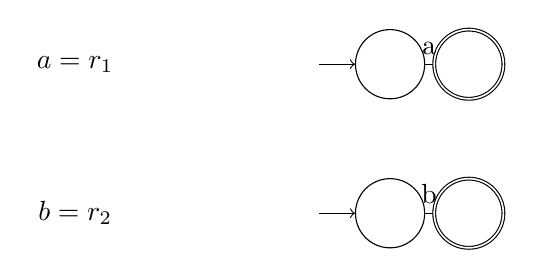
\begin{tikzpicture}
        \node[state, initial, initial text=] (s0) {};
        \node[state, accepting, right of=s0] (s1) {};
        \draw (s0) edge[above] node{a} (s1);
        \path (s0) to ([xshift=-4cm]s0) node(l1){$a = r_1$};

        \node[state, initial, initial text=, below=1cm of s0] (s2) {};
        \node[state, accepting, right of=s2] (s3) {};
        \draw (s2) edge[above] node{b} (s3);
        \path (s2) to ([xshift=-4cm]s2) node(l2){$b = r_2$};

    \end{tikzpicture}
\end{document}